This subsection presents the design of the deployment mechanism to bring the inflatable from its stowed to its deployed configuration. It is key that this action is performed with maximum reliability, since deceleration of the entry vehicle and thereby mission success hinges on the aerodynamic surface area provided by the inflatable decelerator. This design comprises selection of a \acrfull{hdrm}, a canopy to protect the inflatable during interplanetary transfer and its detachment, and deployment.

Deployment of inflatables can be performed either by unrolling, unfolding or deploying a strut \cite[p.222-227]{Jenkins2001}. The former two are deemed impractical for the following reason. Unrolling and unfolding in lateral direction from the centerbody are less package efficient than deploying it as a strut. Unrolling requires a hub about which is rolled and results in multiple toroids stacked together laterally. Unfolding compresses the toroids and thereby also features multiple toroids in lateral direction. Deploying, on the other hand, stretches the sphere cone shape in axial direction and thereby features no more than one toroid in lateral direction. Unrolling and unfolding thus take up more space in radial direction through denser packing in this direction, while deploying stretches the packaging over the axial direction. A key driver for the use of inflatable aeroshells is the launch vehicle constraint on diameter in stowed configuration. By requiring less diameter for aeroshell package, more diameter is left free for the centerbody design. This results in maximum efficiency in the use of available diameter and thereby a more weight-efficient design, since an increase in centerbody diameter is deemed less weight-expensive than an increase in inflatable diameter for a given deployed diameter. This is a result supported by the sensitivity analysis presented in section \ref{sec:strucsens}. 

\begin{figure}[h]
	\centering

	\begin{subfigure}[b]{0.49\textwidth}
		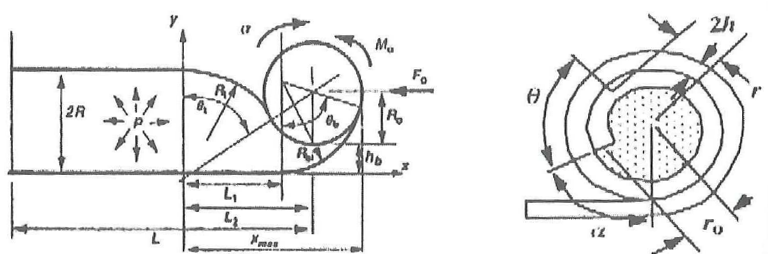
\includegraphics[width=0.96\textwidth]{./Figure/Structure/rot.png}
		\caption{Rotational deployment mechanism}
		\label{fig:rot}
	\end{subfigure}
	\begin{subfigure}[b]{0.49\textwidth}
		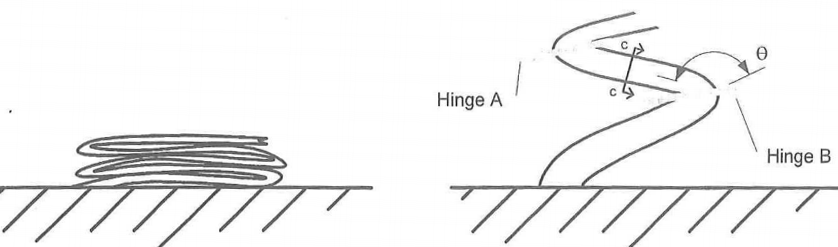
\includegraphics[width=0.96\textwidth]{./Figure/Structure/fold.png}
		\caption{Folding deployment mechanism}
		\label{fig:fold}
	\end{subfigure}
		\begin{subfigure}[b]{1\textwidth}
		\centering
			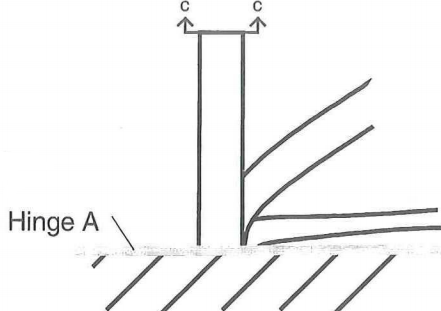
\includegraphics[width=0.3\textwidth]{./Figure/Structure/hinge.png}
			\caption{Hinging deployment mechanism}
			\label{fig:hinge}
		\end{subfigure}
	\caption{Overview of various deployment possibilities \cite{Jenkins2001}}
	\label{fig:dep}
\end{figure}


Moreover, less interference between flexible material is present when deploying the inflatable sphere cone, as opposed to the folding and rolling of the toroids in the other two methods. This decreased amount of interference reduces the unpredictability and thereby increases reliability of the deployment procedure.

Deploying does attachment points at which the outer toroid is held in place in stowed configuration. The axial length over which the inflatable is held in stowed condition is equal to the inflated radius minus the centerbody radius, equal to XXX [m]. Attachment points will therefore be located at the side of the crew module, such that the inflatable is wrapped about the vehicle in stowed condition. 

To initiate deployment events \glspl{hdrm} are used. As deployment is a singular event in time, one-time use is warranted. Reusable mechanisms typically have a larger number of moving parts and thereby a lower reliability than non-reusable mechanisms \footnote{URL: \url{http://www.esa.int/Our_Activities/Space_Engineering_Technology/Mechanisms/Hold-Down_and_Separation_Systems}. Accessed: 04-06-2015}. Reliability is key, since deployment of the aeroshell is of singular importance to aerodynamically decelerate the vehicle. To this end, pyro cutters are the pre-eminent solution by their high and proven reliability in space operations, low weight and shock imparted to the vehicle. Example cutters are Chemring Hi-Shear cutters, applied in multiple space missions, such as the Mars observer mission \footnote{URL: \url{http://www.hstc.com/Products/OrdnanceProducts/CuttersBoltRodandCab/}. Accessed: 08-06-2015}. These possess a weight in the order of one hundred grammes. For their criticality in mission success, redundancy of \glspl{hdrm} is key and at each location at least two cutters are required to be present.

